\chapter{Testing e valutazione delle prestazioni del sistema} 

\begin{citazione}
In questa sezione, il sistema sarà messo alla prova, misurando le sue prestazioni in termini di velocità, efficienza e affidabilità. Questo permetterà di individuare eventuali aree di miglioramento e di ottimizzare il sistema per garantire la migliore esperienza possibile agli utenti finali.
\end{citazione}
\newpage

\section{Progettazione dei test}
Come è stato spiegato nel capitolo \emph{Progettazione}, alla base di ogni esperimento è stato definito un preciso \emph{flusso di dati} avente dei requisiti di \emph{QoS}. Sono stati presi in considerazione i flussi che al giorno d'oggi sono maggiormente utilizzati nell'ambito delle comunicazioni e di fornitura di determinati servizi web based. Sotto sono riportati i flussi che sono stati presi in considerazione per gli esperimenti da eseguire; ogni flusso ha il compito di simulare uno specifico servizio nel modo più fedele possibile: 
\newline
\begin{itemize}
    \item Flusso UDP per misurare il \emph{throughput} massimo;
    \item Flusso TCP per misurare il \emph{throughput} massimo;
    \item Flusso UDP per simulare il protocollo \emph{VoIP};
    \item Flusso per simulare uno \emph{streaming video};
    \item Flusso per simulare un \emph{trasferimento massivo}.
\end{itemize} 

\section{Implementazione dei flussi con iPerf}
Nel paragrafo precedente sono stati progettati i diversi flussi di dati da utilizzare per i vari test da eseguire; per la realizzazione vera e propria si è scelto di utilizzare \emph{iPerf} il quale permette di poter simulare un flusso di dati in maniera molto precisa tramite l'utilizzo di numerosi \emph{flag} e di poter gestire lo scambio di dati tra un \emph{server} ed un \emph{client} i quali eseguono entrambi il tool. Sotto è riportata la definizione esatta dei comandi per simulare i flussi:
\begin{itemize}
    \item \fcolorbox{black}{red!5}{.\textbackslash iperf3 -c 10.66.66.1 -p 2020 -u -b 0 -n 512M --get-server-output;} \newline
    Questo comando simula l'invio di 512 MB tramite il protocollo di rete UDP, utilizzando tutta la banda disponibile.
    \item \fcolorbox{black}{red!5}{.\textbackslash iperf3 -c 10.66.66.1 -p 2020 -P 10 -b 0 -w 100k --get-server-output;} \newline
    Questo flusso simula l'invio di pacchetti TCP utilizzando dieci connessioni parallele verso il server ed la massima banda disponibile.
    \item \fcolorbox{black}{red!5}{.\textbackslash iperf3 -c 10.66.66.1 -u -p 2020 -S 0x28 -l 78 -b 100K --get-server-output;} \newline
    Questo flusso simula l'invio di pacchetti UDP appartenenti ad un flusso di dati di tipo VoIP.
    \item \fcolorbox{black}{red!5}{.\textbackslash iperf3 -c 10.66.66.1 -p 2020 -S 32 -M 1460B --get-server-output;} \newline
    Questo flusso simula l'invio di pacchetti TCP appartenenti ad un flusso di streaming video.
    \item .\textbackslash \fcolorbox{black}{red!5}{.\textbackslash iperf3 -c 10.66.66.1 -p 2020 -S 10 -M 1460B -b 0 --get-server-output;} \newline
    Questo flusso simula l'invio di pacchetti TCP appartenenti ad un flusso bulk data cioè di trasferimento di massa.
\end{itemize}
\subsubsection{Dettagli sui flag utilizzati}
Al fine di comprendere a pieno come sono stati simulati i diversi flussi di dati scambiati negli esperimenti tra client e server, è importante capire il significato dei \emph{flag} utilizzati:
\begin{itemize}
    \item \emph{-c}: Indirizzo dell'host che esegue iPerf server;
    \item \emph{-p}: Porta in ascolto di iPerf server;
    \item \emph{-u}: Flusso di tipo UDP;
    \item \emph{-b}: Banda disponibile per il trasferimento. 0 indica che la banda è massima;
    \item \emph{-n}: Quantità di byte da inviare durante il test;
    \item \emph{-P}: Numero di connessioni parallele del client;
    \item \emph{-S}: Assegna ai pacchetti una determinata priorità per simulare i pacchetti di un preciso protocollo applicativo;
    \item \emph{-M}: Grandezza massima del singolo pacchetto TCP;
    \item \emph{--get-server-output}: L'output del test viene visualizzato anche sul client.
\end{itemize}

\section{Definizione metriche di valutazione}
Arrivati a questo punto del lavoro è molto importante capire sulla base di quali \emph{parametri} effettuare la valutazione del sistema realizzato in modo da poter stabilire con certezza l'efficacia di esso. A tal proposito, è stato scelto di rendere le valutazioni degli esperimenti del tutto indipendenti tra loro; in particolare i diversi esperimenti sono stati valutati in base ai valori assunti principalmente dai due seguenti parametri:

\begin{itemize}
    \item \emph{Bitrate}: Indica la quantità di informazioni che sono state trasferite in un'unica unità di tempo;
    \item \emph{Trasferimento}: Indica la quantità di informazioni trasferite durante l'esecuzione dell'intero test.
\end{itemize}

I parametri sopracitati sono di fondamentale importanza affinché si possa stabilire se le \emph{condizioni di rete}, derivanti anche dall'utilizzo o meno di uno dei protocolli VPN, siano adatte per consentire il corretto impiego dei flussi stabiliti.

\section{Esecuzione degli esperimenti e analisi dei risultati}
Il passo successivo è quello di proseguire con l'esecuzione degli esperimenti prefissati in modo da poter raccogliere i dati di output e poterli utilizzare per la generazione di \emph{grafici} da utilizzare come strumento di ausilio all'analisi degli output stessi. Al fine di evitare ripetizioni superflue è stato evitato di trattare ogni singola esecuzione di ogni test per cui nel paragrafo successivo è riportato un singolo campione di esecuzione che rispecchia la struttura di tutte le altre indipendentemente dal protocollo VPN utilizzato. I dati di output di tutte le esecuzioni dei test sono presenti nel progetto \emph{GitHub} \cite{pro}.

\subsection{Esempio di esecuzione test}
Nel seguente sottoparagrafo è riportato un esempio di una singola esecuzione del test \emph{numero 1} tra il sistema TurtleVPN ed un client, avente sistema operativo \emph{Windows 11}, il quale invia il flusso di dati in modo da poter ricevere i risultati di output. Nella figura 6.1 è rappresentata l'esecuzione del comando per fare in modo che TurtleVPN possa ricevere il flusso di dati prestabilito che sarà inviato dal client, come in figura 6.2, il quale riceverà anche l'output dell'esecuzione. Ogni esperimento è stato eseguito allo stesso modo indipendentemente dal protocollo VPN impiegato. Da come si nota dalla figura 6.2, l'output del test è suddiviso in intervalli i quali sono numericamente differenti in base al tipo di flusso simulato.

\begin{figure}[h] 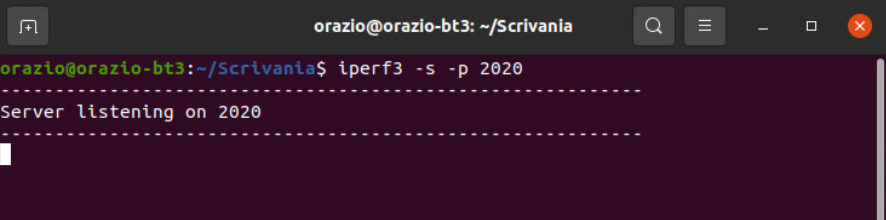
\includegraphics[width=0.6\textwidth] {Tesi magistrale/capitoli/images/iPerf server.png}
\centering
\caption{Comando iPerf server.}
\end{figure}

\begin{figure}[h] 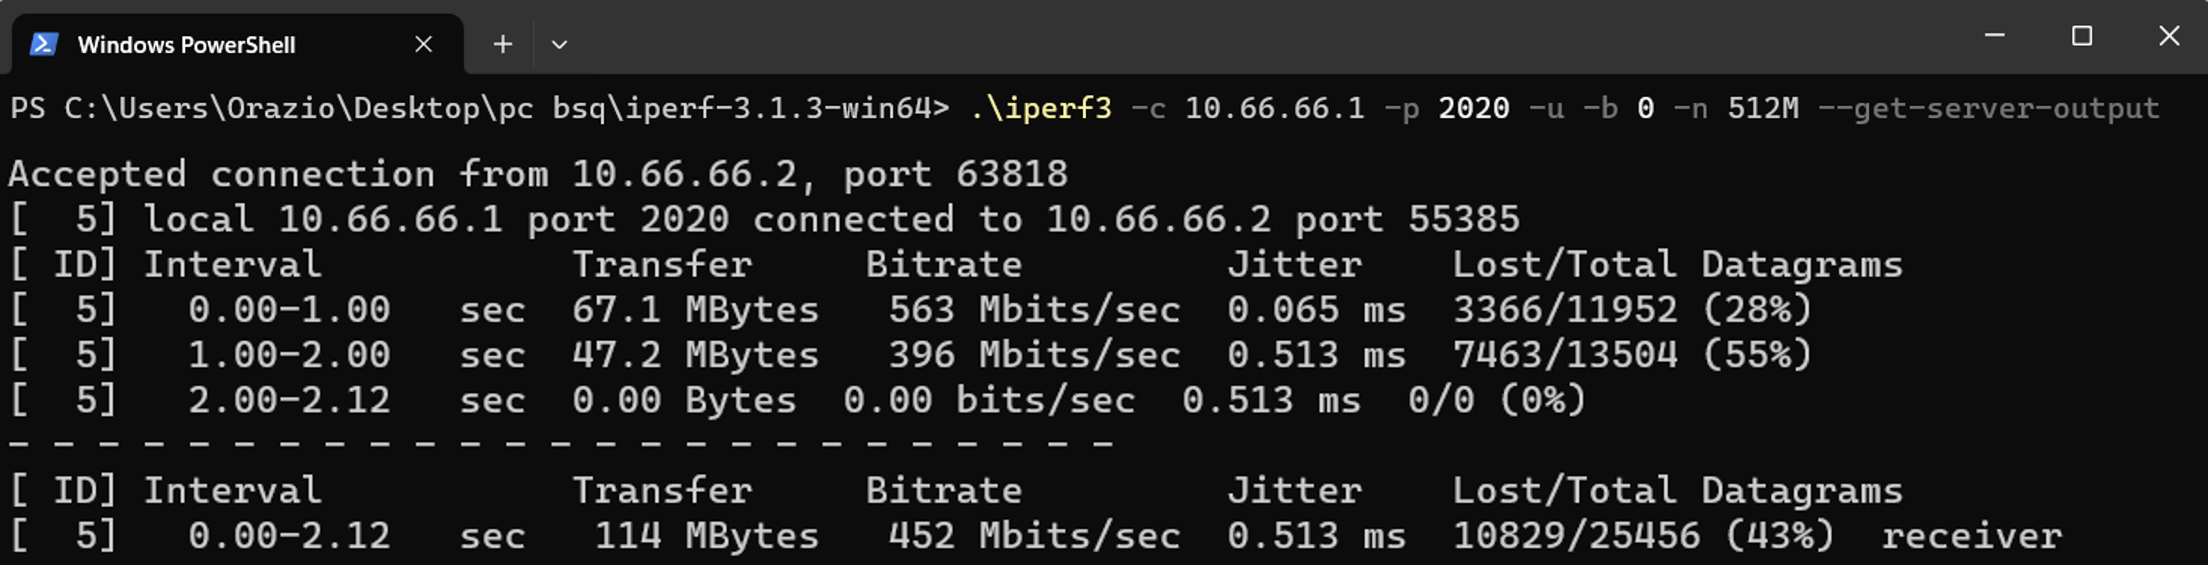
\includegraphics[width=0.7\textwidth] {Tesi magistrale/capitoli/images/iPerf client.png}
\centering
\caption{Comando iPerf client.}
\end{figure}

\newpage

Sulla base degli output ottenuti dalle varie esecuzioni di ogni test, saranno estrapolate le considerazioni sui protocolli VPN, grazie anche ai grafici generati a partire proprio dai dati di output dei test.

\section{Analisi dei risultati}
Analizziamo ora i risultati ottenuti dai test; in particolare i grafici riguardano i parametri \emph{bitrate} e \emph{transfer} ottenuti in output da ogni esecuzione. Per ogni esperimento sono quindi stati creati \emph{due} grafici per ognuna delle \emph{dieci} esecuzioni del test in modo da avere una visione chiara dell'andamento dell'esperimento, inoltre per ogni esperimento sono stati generati anche due grafici ad istogramma rappresentanti \emph{bitarte} e \emph{transfer} medio. Visto che ogni esperimento è stato eseguito con diversi protocolli VPN, si eviterà di mostrare tutti i grafici affinché si possa cogliere il senso di ogni esperimento; il set di grafici completo è presente nel progetto \emph{GitHub} \cite{pro}.

\newpage
\subsection{Primo esperimento}
L'esperimento in questione riguarda l'invio di 512 MB tramite l'utilizzo del protocollo UDP, sfruttando tutta la banda di rete disponibile.

\subsubsection{Grafici esperimento senza VPN}

\begin{figure}[h] 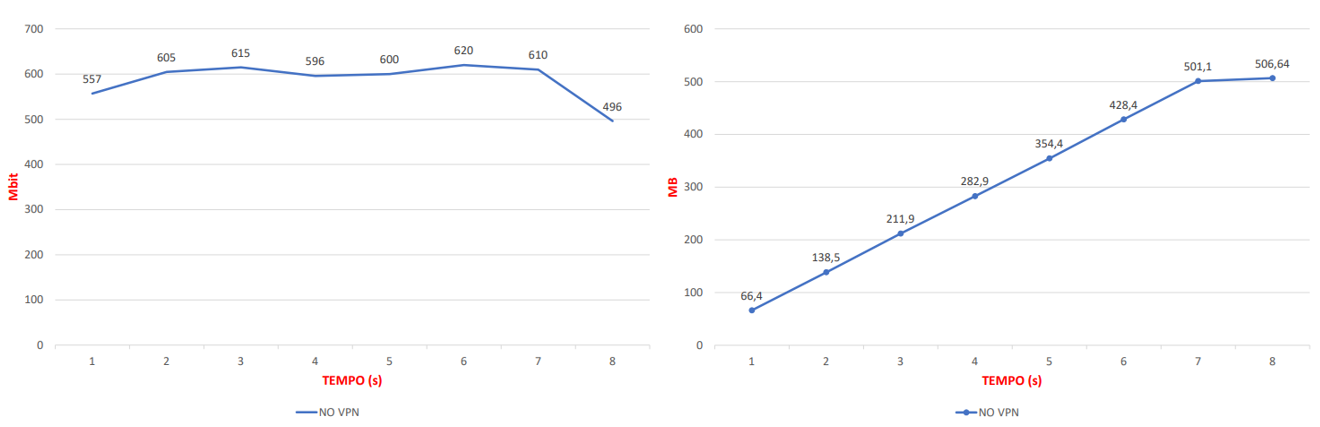
\includegraphics[width=0.9\textwidth] {Tesi magistrale/capitoli/images/1.png}
\centering
\caption{Grafici 1° esecuzione.}
\end{figure}

\begin{figure}[h] 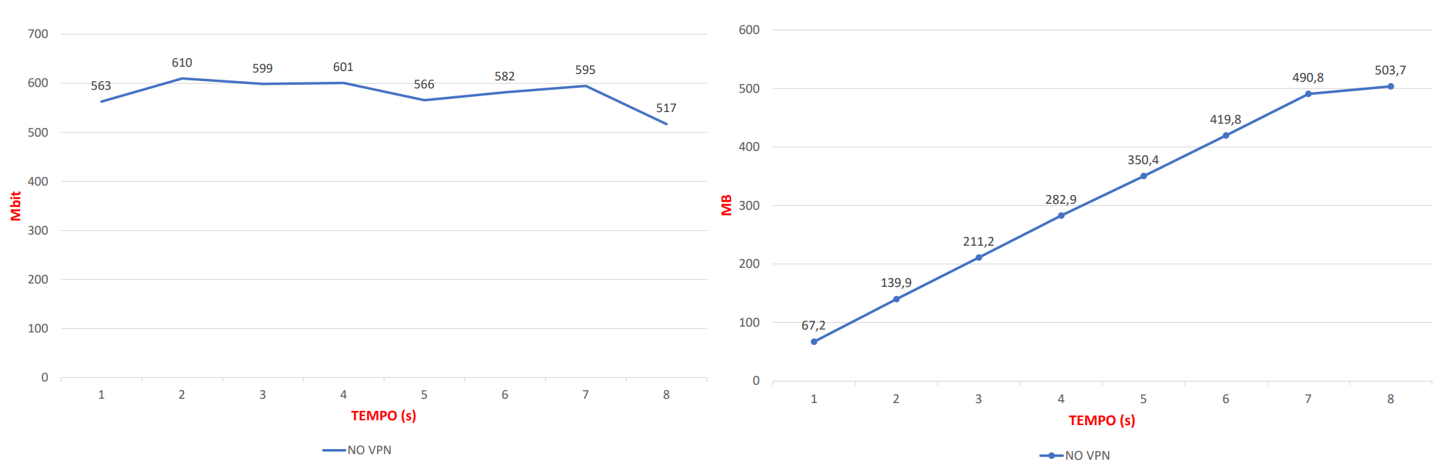
\includegraphics[width=0.9\textwidth] {Tesi magistrale/capitoli/images/2.png}
\centering
\caption{Grafici 5° esecuzione.}
\end{figure}

\begin{figure}[h] 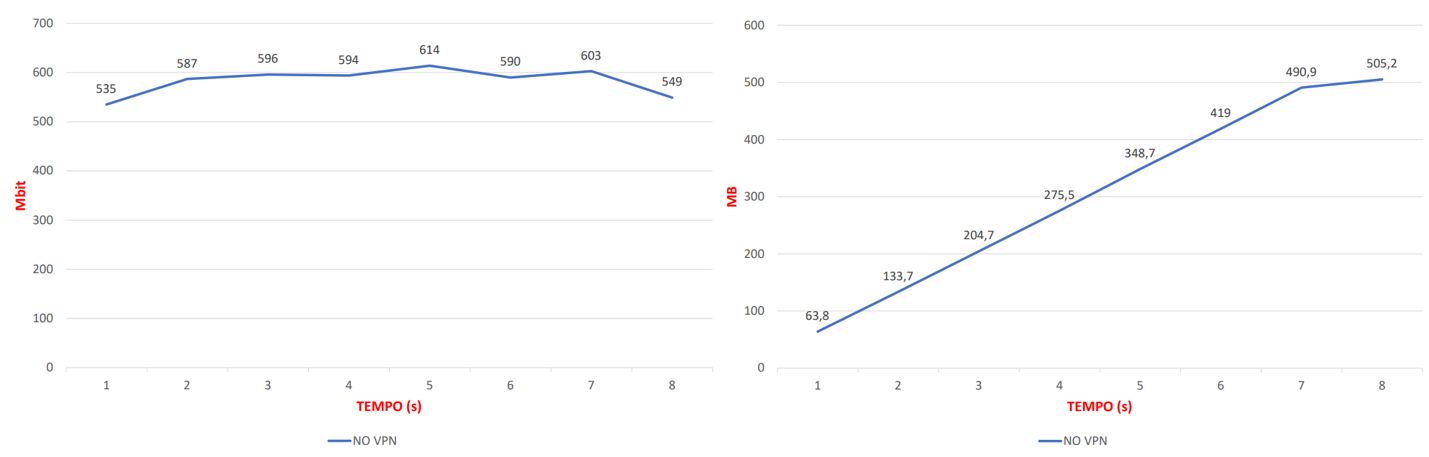
\includegraphics[width=0.9\textwidth] {Tesi magistrale/capitoli/images/3.png}
\centering
\caption{Grafici 10° esecuzione.}
\end{figure}

\newpage
\subsubsection{Grafici esperimento con WireGuard standard}

\begin{figure}[h] 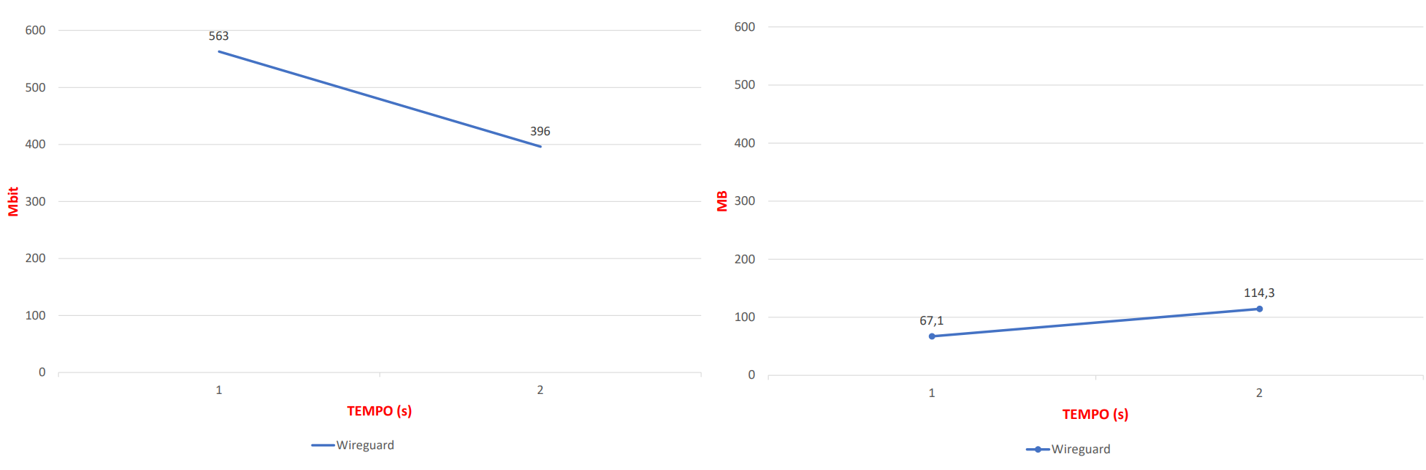
\includegraphics[width=0.9\textwidth] {Tesi magistrale/capitoli/images/4.png}
\centering
\caption{Grafici 1° esecuzione.}
\end{figure}

\begin{figure}[h] 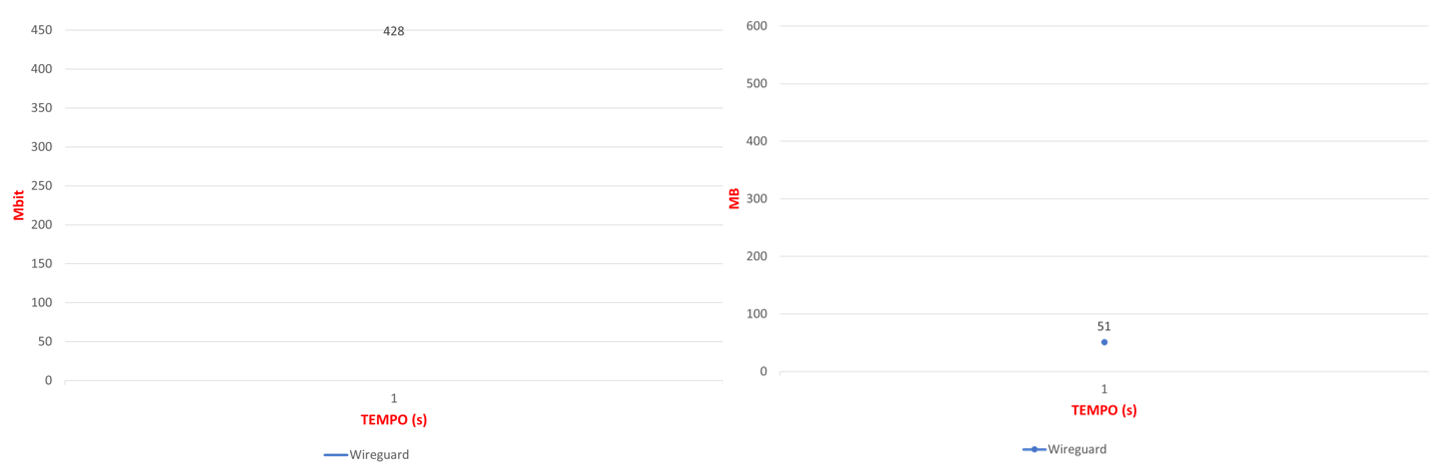
\includegraphics[width=0.9\textwidth] {Tesi magistrale/capitoli/images/5.png}
\centering
\caption{Grafici 5° esecuzione.}
\end{figure}

\begin{figure}[h] 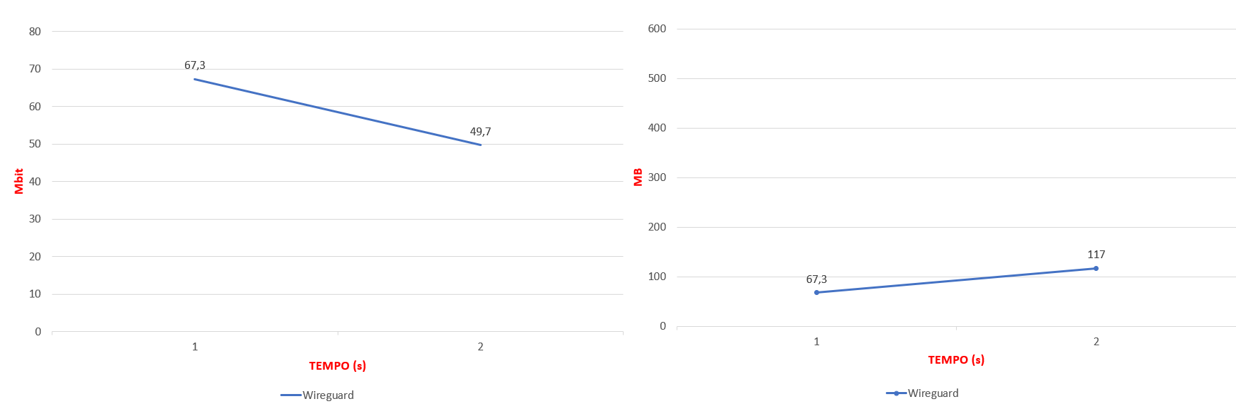
\includegraphics[width=0.9\textwidth] {Tesi magistrale/capitoli/images/6.png}
\centering
\caption{Grafici 10° esecuzione.}
\end{figure}

\newpage
\subsubsection{Grafici esperimento con WireGuard PQ}

\begin{figure}[h] 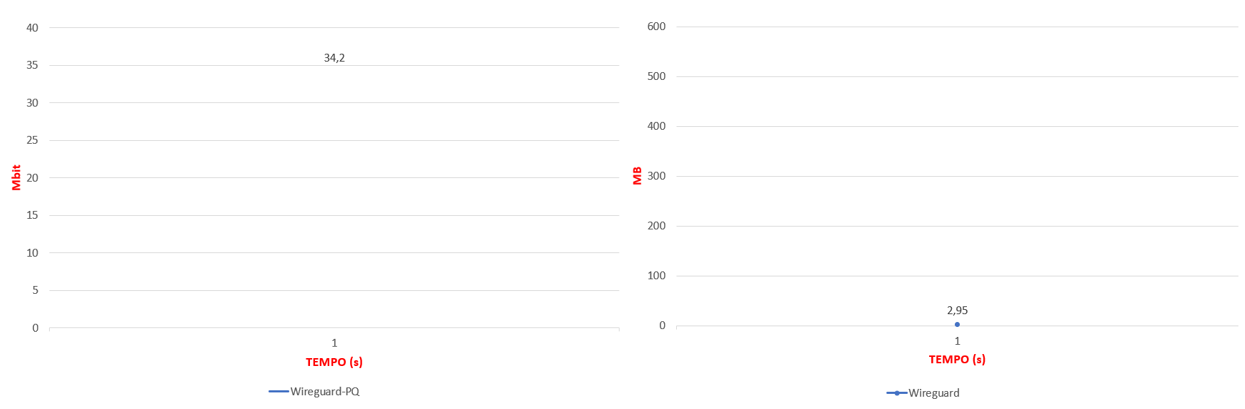
\includegraphics[width=0.9\textwidth] {Tesi magistrale/capitoli/images/7.png}
\centering
\caption{Grafici 1° esecuzione.}
\end{figure}

\begin{figure}[h] 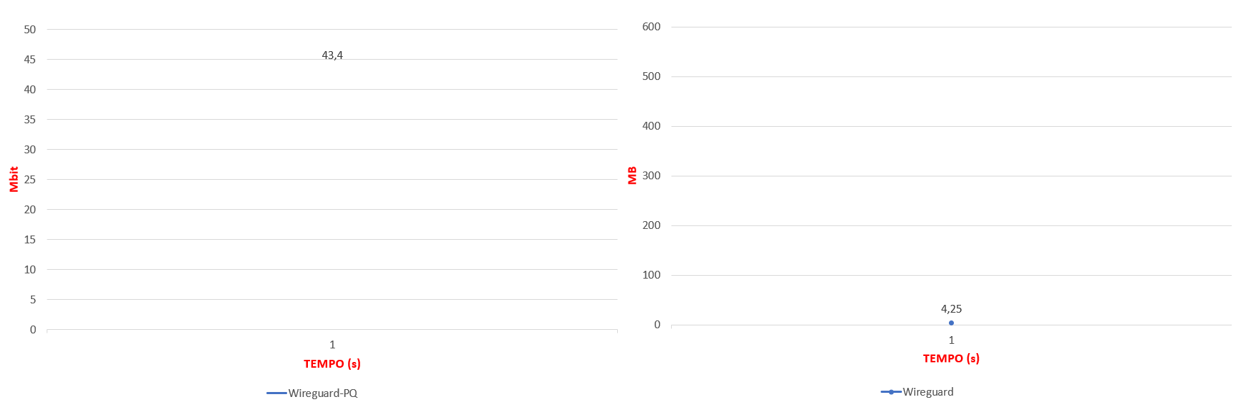
\includegraphics[width=0.9\textwidth] {Tesi magistrale/capitoli/images/8.png}
\centering
\caption{Grafici 5° esecuzione.}
\end{figure}

\begin{figure}[h] 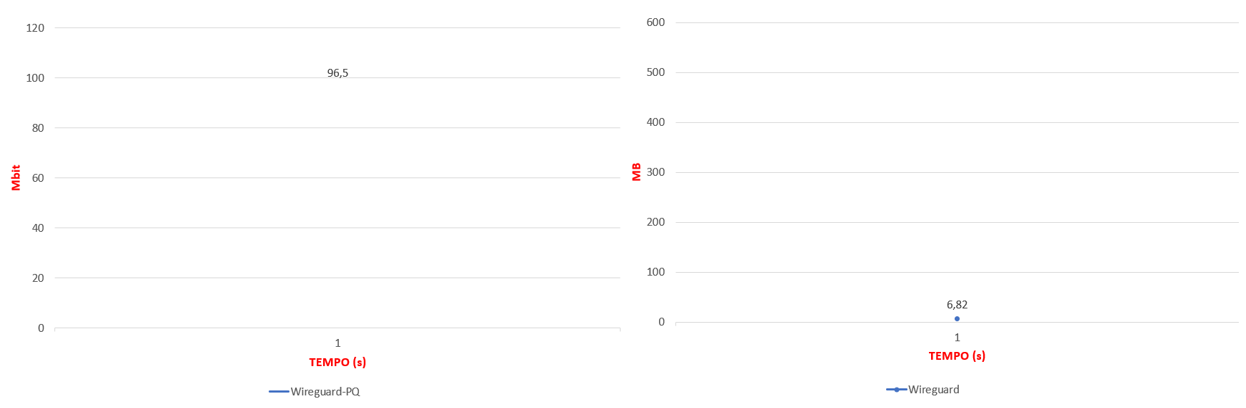
\includegraphics[width=0.9\textwidth] {Tesi magistrale/capitoli/images/9.png}
\centering
\caption{Grafici 10° esecuzione.}
\end{figure}

\newpage
\subsubsection{Grafici esperimento con OpenVPN}

\begin{figure}[h] 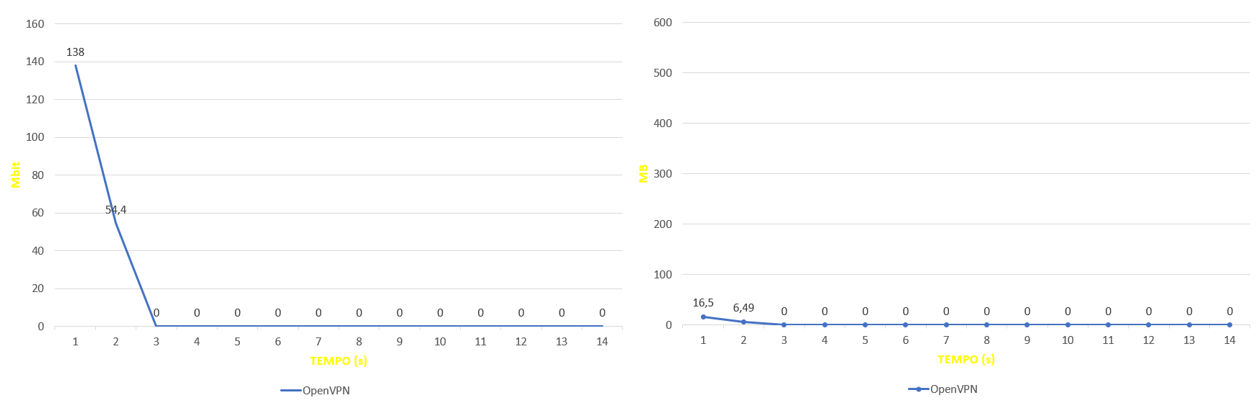
\includegraphics[width=0.9\textwidth] {Tesi magistrale/capitoli/images/10.png}
\centering
\caption{Grafici 1° esecuzione.}
\end{figure}

\begin{figure}[h] 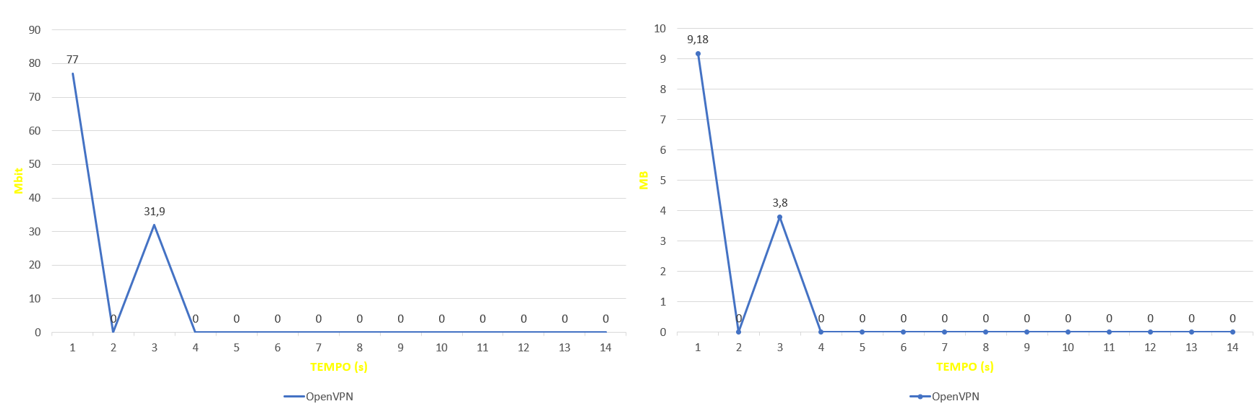
\includegraphics[width=0.9\textwidth] {Tesi magistrale/capitoli/images/11.png}
\centering
\caption{Grafici 5° esecuzione.}
\end{figure}

\begin{figure}[h] 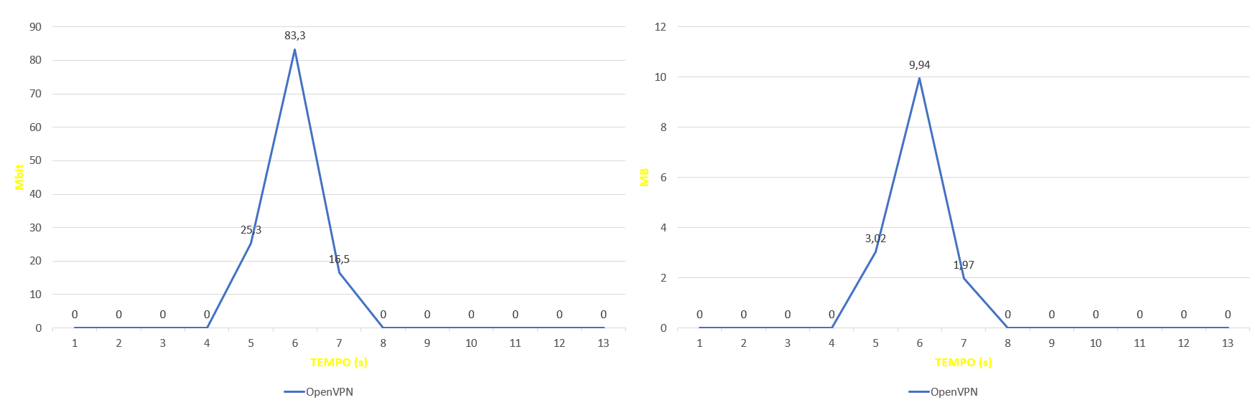
\includegraphics[width=0.9\textwidth] {Tesi magistrale/capitoli/images/12.png}
\centering
\caption{Grafici 10° esecuzione.}
\end{figure}

\newpage
\subsubsection{Grafici riassuntivi}

\begin{figure}[h] 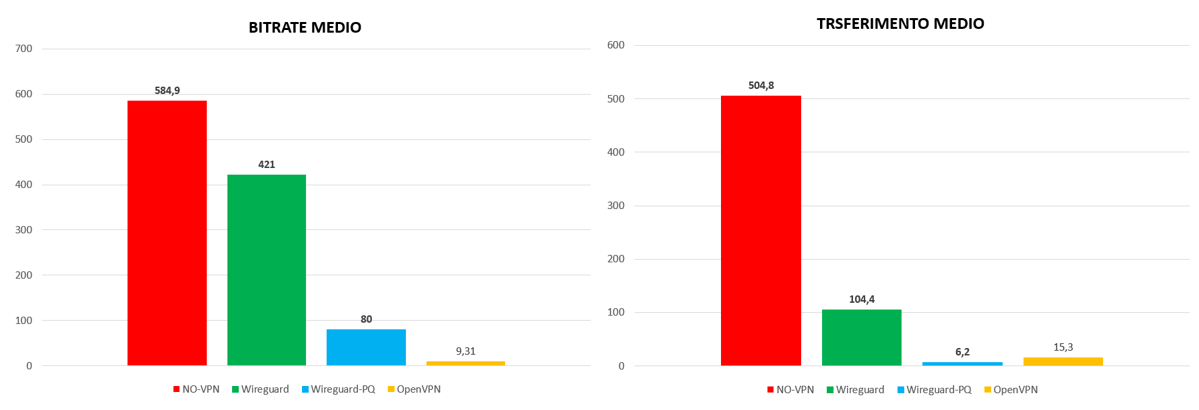
\includegraphics[width=1\textwidth] {Tesi magistrale/capitoli/images/13.png}
\centering
\caption{Grafici riassuntivi.}
\end{figure}

\subsubsection{Esito primo esperimento}
Dai grafici si può notare che ovviamente l'esperimento restituisce i risultati migliori quando nessun protocollo VPN è attivo; mentre tra le diverse VPN testate quella che si comporta meglio è sicuramente \emph{WireGuard standard} il quale offre prestazioni migliori almeno in questo esperimento. 

\newpage
\subsection{Secondo esperimento}
Il secondo esperimento riguarda l'invio di numerosi pacchetti tramite l'utilizzo del protocollo TCP e di dieci connessioni parallele verso il server iPerf in modo da poter stabilire principalmente il throughput massimo raggiungibile.
\subsubsection{Grafici esperimento senza VPN}

\begin{figure}[h] 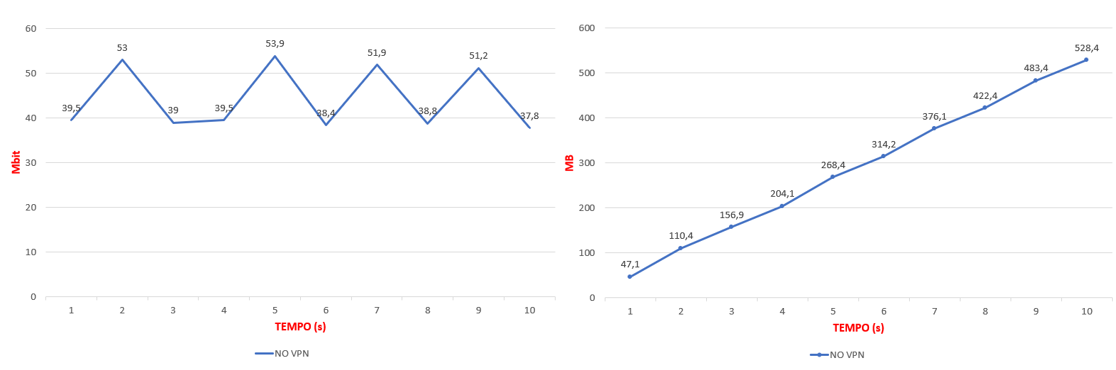
\includegraphics[width=0.9\textwidth] {Tesi magistrale/capitoli/images/14.png}
\centering
\caption{Grafici 1° esecuzione.}
\end{figure}

\begin{figure}[h] 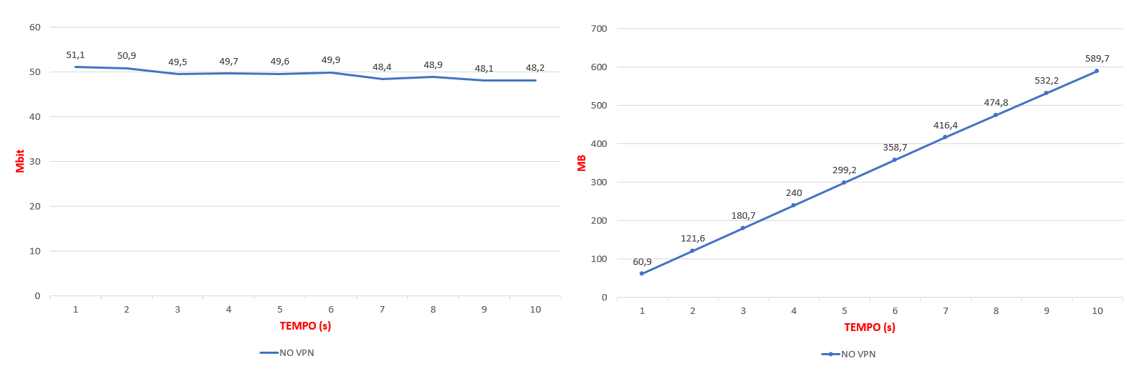
\includegraphics[width=0.9\textwidth] {Tesi magistrale/capitoli/images/15.png}
\centering
\caption{Grafici 5° esecuzione.}
\end{figure}

\begin{figure}[h] 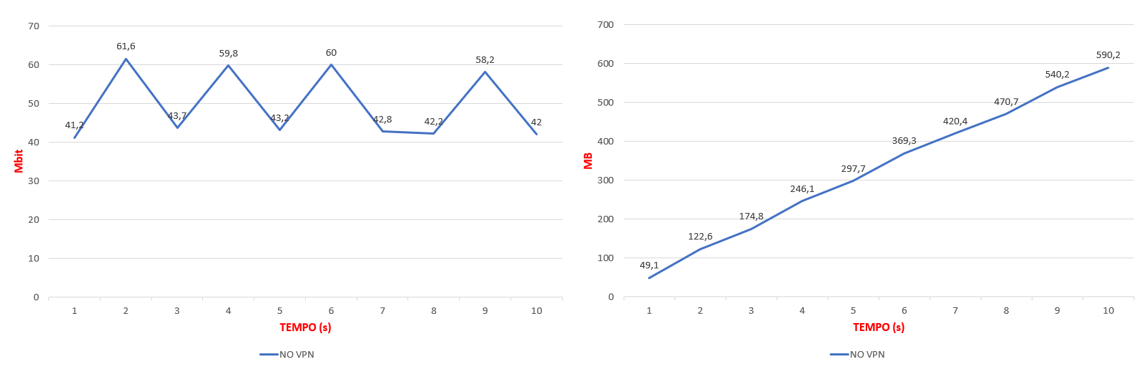
\includegraphics[width=0.9\textwidth] {Tesi magistrale/capitoli/images/16.png}
\centering
\caption{Grafici 10° esecuzione.}
\end{figure}

\newpage
\subsubsection{Grafici esperimento con WireGuard standard}

\begin{figure}[h] 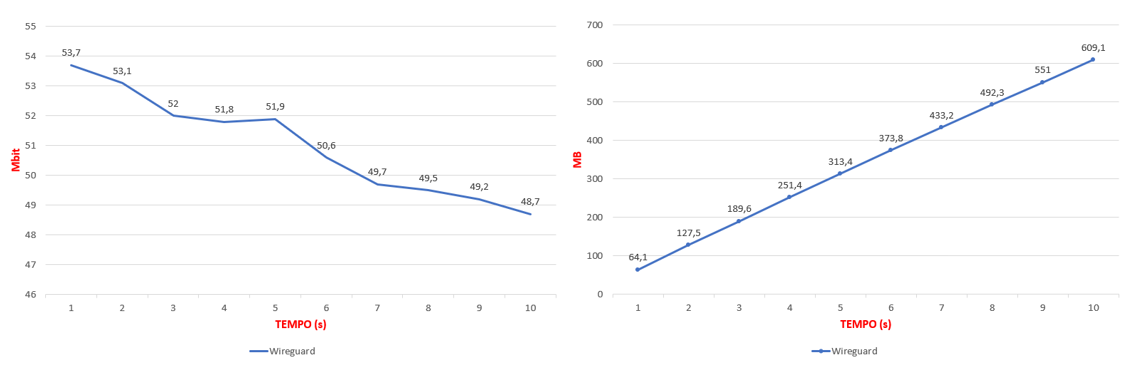
\includegraphics[width=0.9\textwidth] {Tesi magistrale/capitoli/images/17.png}
\centering
\caption{Grafici 1° esecuzione.}
\end{figure}

\begin{figure}[h] 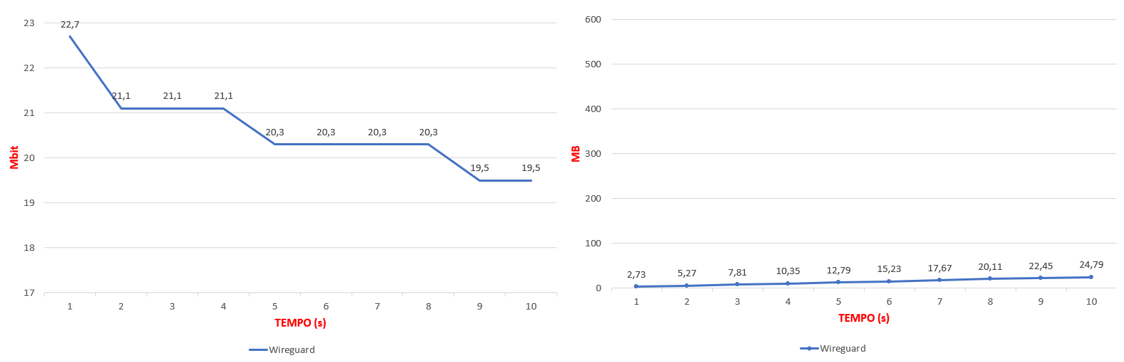
\includegraphics[width=0.9\textwidth] {Tesi magistrale/capitoli/images/18.png}
\centering
\caption{Grafici 5° esecuzione.}
\end{figure}

\begin{figure}[h] 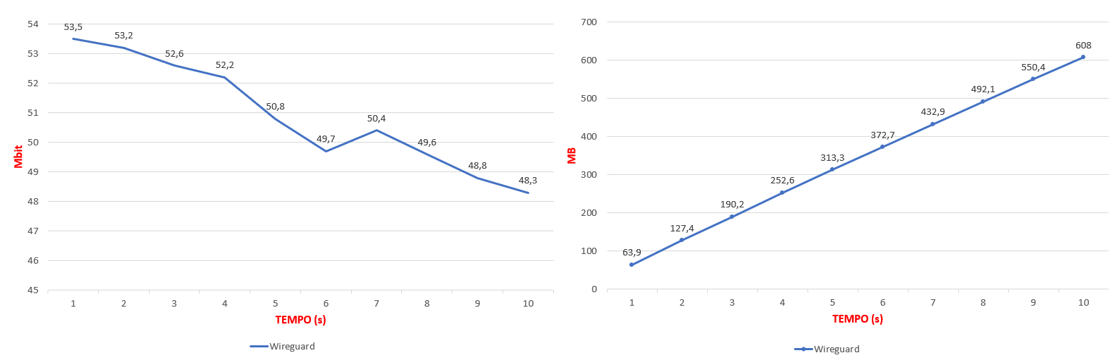
\includegraphics[width=0.9\textwidth] {Tesi magistrale/capitoli/images/19.png}
\centering
\caption{Grafici 10° esecuzione.}
\end{figure}

\newpage
\subsubsection{Grafici esperimento con WireGuard PQ}

\begin{figure}[h] 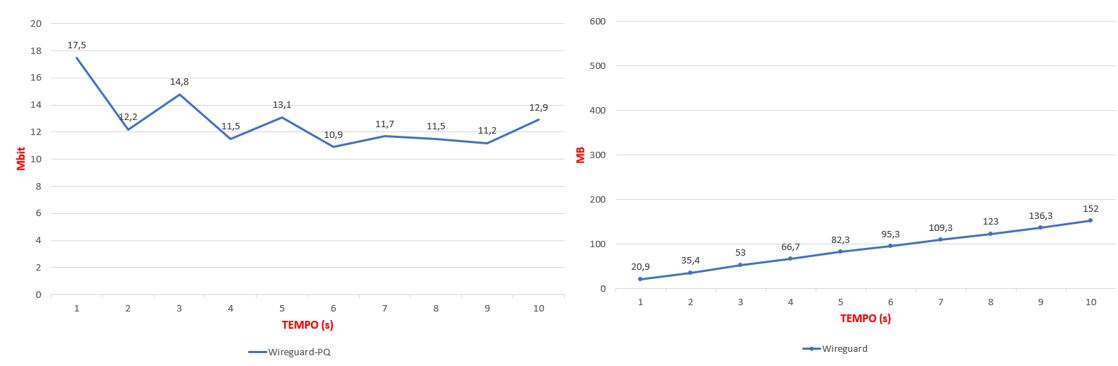
\includegraphics[width=0.9\textwidth] {Tesi magistrale/capitoli/images/20.png}
\centering
\caption{Grafici 1° esecuzione.}
\end{figure}

\begin{figure}[h] 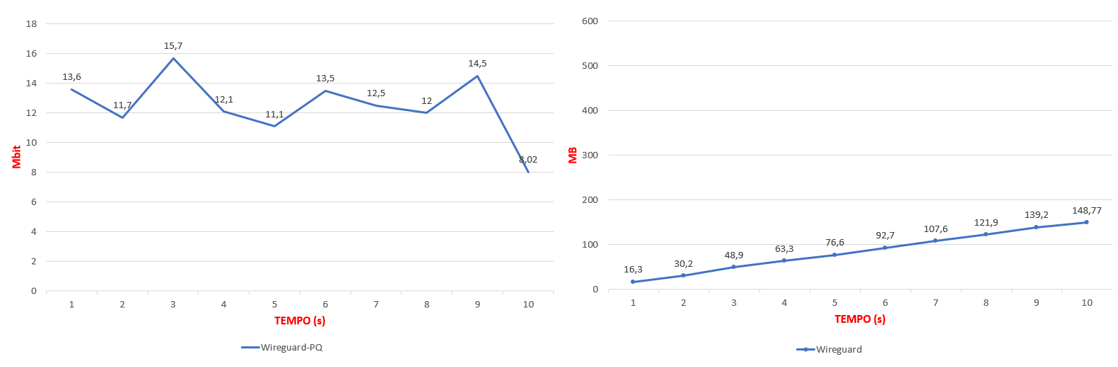
\includegraphics[width=0.9\textwidth] {Tesi magistrale/capitoli/images/21.png}
\centering
\caption{Grafici 5° esecuzione.}
\end{figure}

\begin{figure}[h] 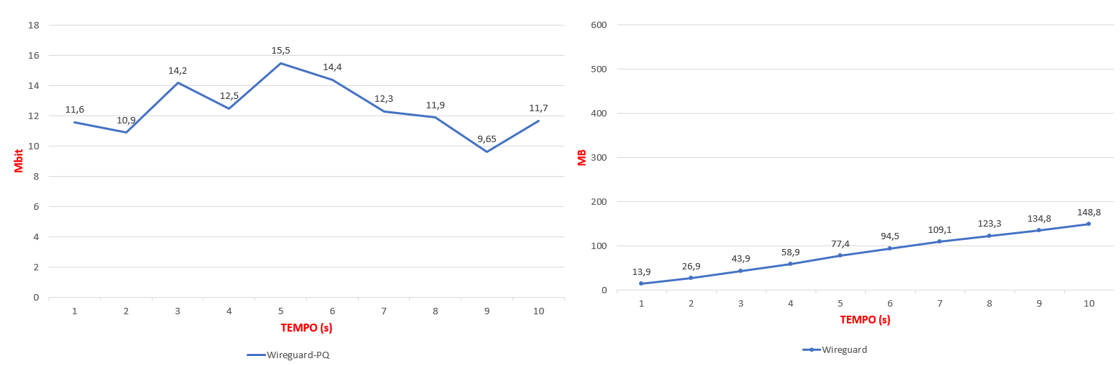
\includegraphics[width=0.9\textwidth] {Tesi magistrale/capitoli/images/22.png}
\centering
\caption{Grafici 10° esecuzione.}
\end{figure}

\newpage
\subsubsection{Grafici esperimento con OpenVPN}

\begin{figure}[h] 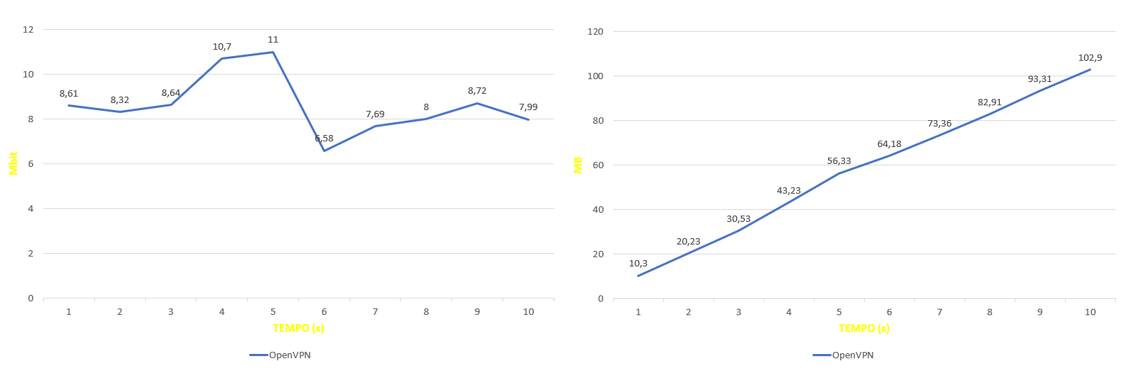
\includegraphics[width=0.9\textwidth] {Tesi magistrale/capitoli/images/23.png}
\centering
\caption{Grafici 1° esecuzione.}
\end{figure}

\begin{figure}[h] 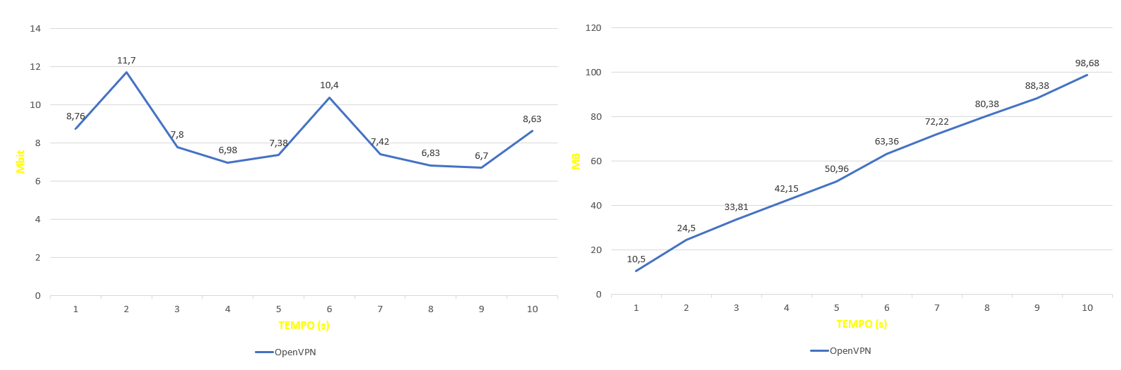
\includegraphics[width=0.9\textwidth] {Tesi magistrale/capitoli/images/24.png}
\centering
\caption{Grafici 5° esecuzione.}
\end{figure}

\begin{figure}[h] 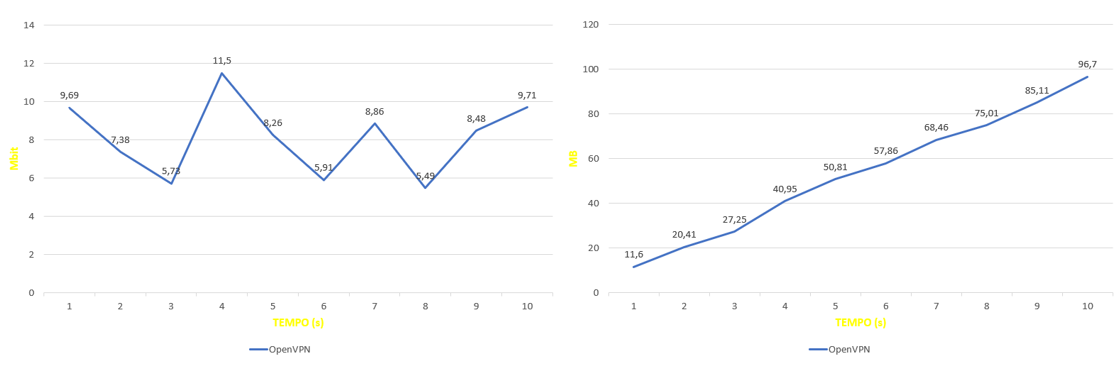
\includegraphics[width=0.9\textwidth] {Tesi magistrale/capitoli/images/25.png}
\centering
\caption{Grafici 10° esecuzione.}
\end{figure}

\newpage
\subsubsection{Grafici riassuntivi}

\begin{figure}[h] 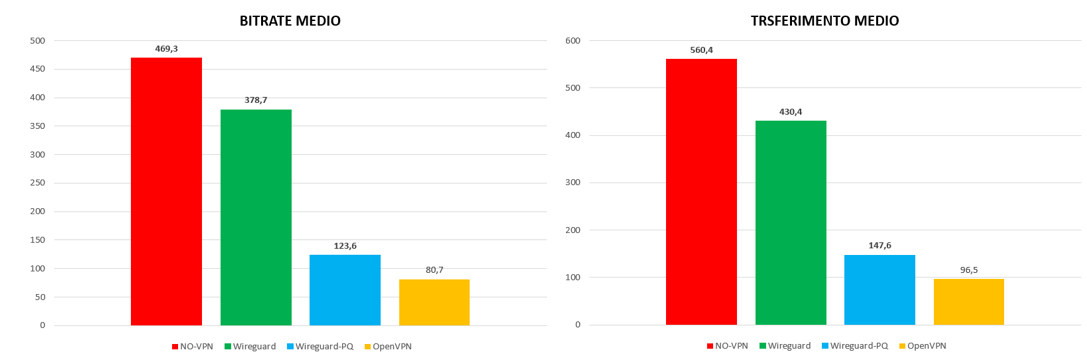
\includegraphics[width=1\textwidth] {Tesi magistrale/capitoli/images/26.png}
\centering
\caption{Grafici riassuntivi.}
\end{figure}

\subsubsection{Esito secondo esperimento}
Come nel primo esperimento, anche in questo caso è ovvio che l'esito sia a favore dell'esecuzione senza impiego di protocolli VPN anche se il divario con essi è abbastanza trascurabile, soprattutto se si considera l'output del test con l'utilizzo di \emph{WireGuard standard}.

\newpage
\subsection{Terzo esperimento}
Questo esperimento riguarda la simulazione di invio di un flusso di dati di livello \emph{applicativo}, in particolare del protocollo \emph{VoIP}.  
\subsubsection{Grafici esperimento senza VPN}

\begin{figure}[h] 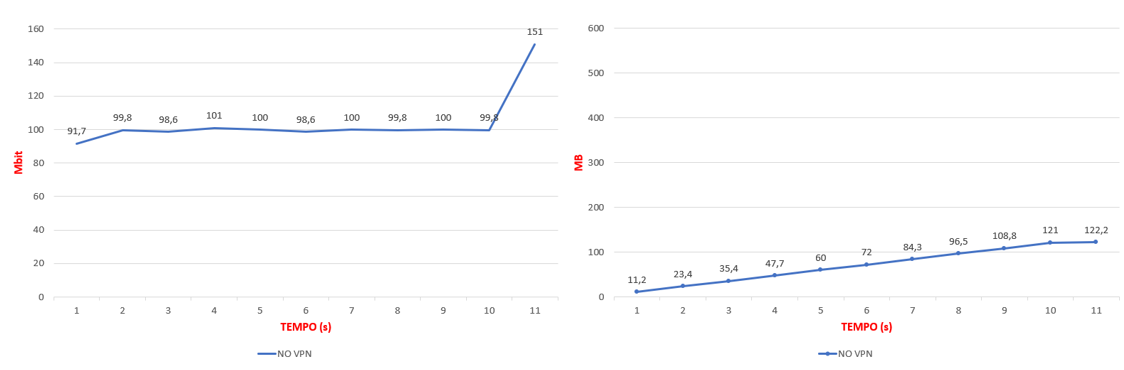
\includegraphics[width=0.9\textwidth] {Tesi magistrale/capitoli/images/27.png}
\centering
\caption{Grafici 1° esecuzione.}
\end{figure}

\begin{figure}[h] 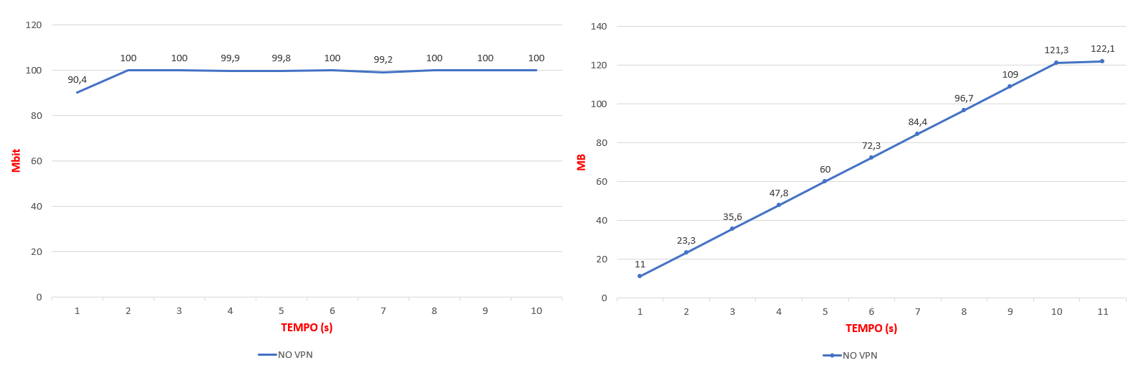
\includegraphics[width=0.9\textwidth] {Tesi magistrale/capitoli/images/28.png}
\centering
\caption{Grafici 5° esecuzione.}
\end{figure}

\begin{figure}[h] 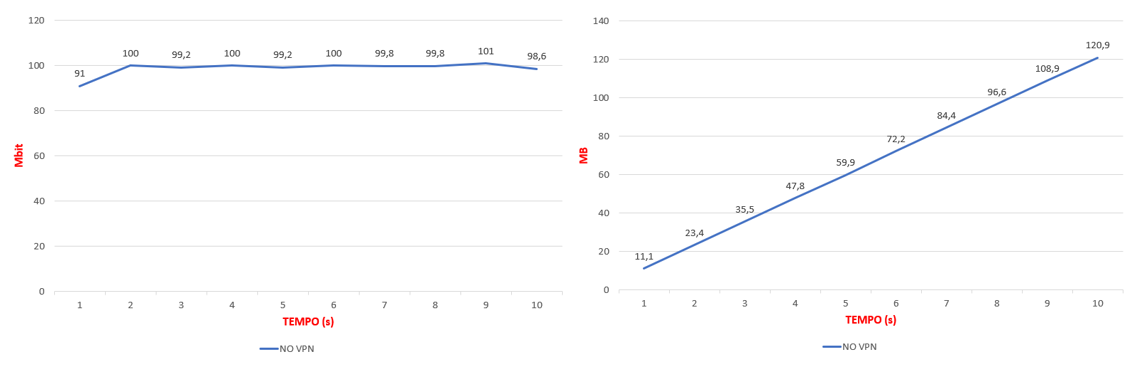
\includegraphics[width=0.9\textwidth] {Tesi magistrale/capitoli/images/29.png}
\centering
\caption{Grafici 10° esecuzione.}
\end{figure}

\newpage
\subsubsection{Grafici esperimento con WireGuard standard}

\begin{figure}[h] 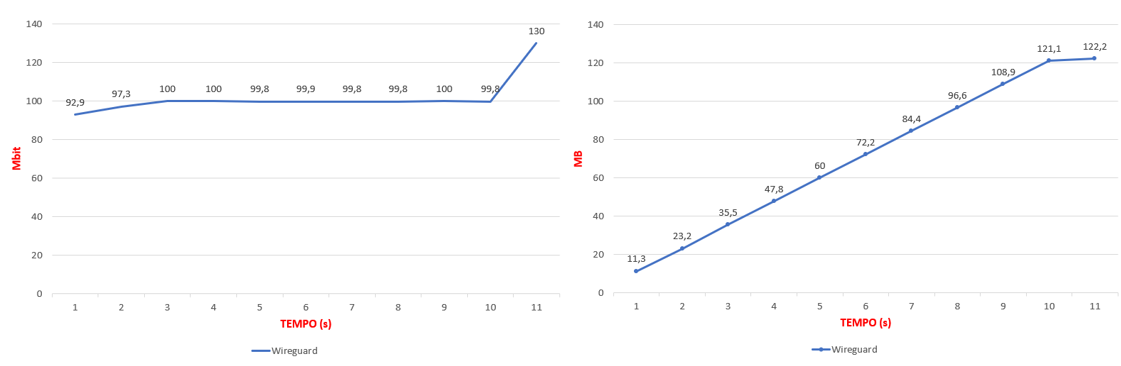
\includegraphics[width=0.9\textwidth] {Tesi magistrale/capitoli/images/30.png}
\centering
\caption{Grafici 1° esecuzione.}
\end{figure}

\begin{figure}[h] 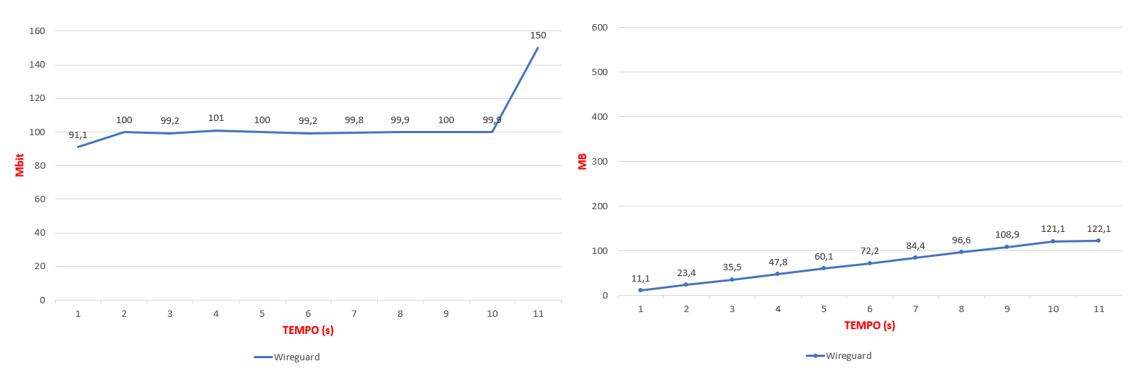
\includegraphics[width=0.9\textwidth] {Tesi magistrale/capitoli/images/31.png}
\centering
\caption{Grafici 5° esecuzione.}
\end{figure}

\begin{figure}[h] 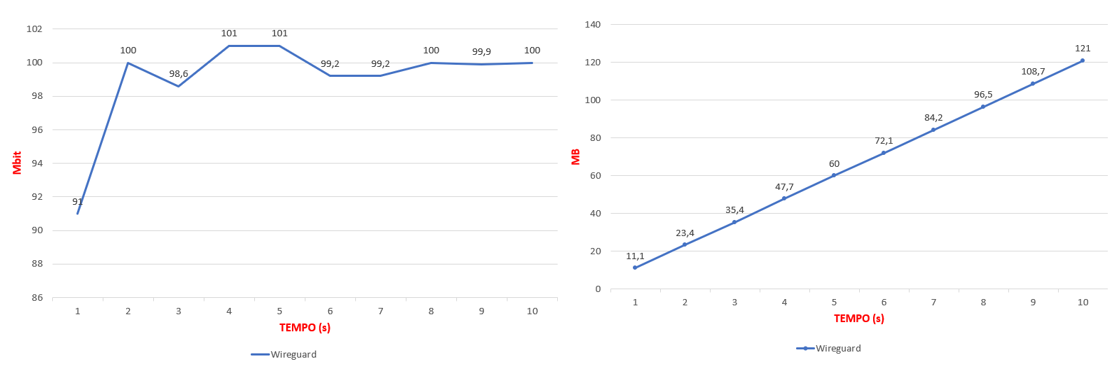
\includegraphics[width=0.9\textwidth] {Tesi magistrale/capitoli/images/32.png}
\centering
\caption{Grafici 10° esecuzione.}
\end{figure}

\newpage
\subsubsection{Grafici esperimento con WireGuard PQ}

\begin{figure}[h] 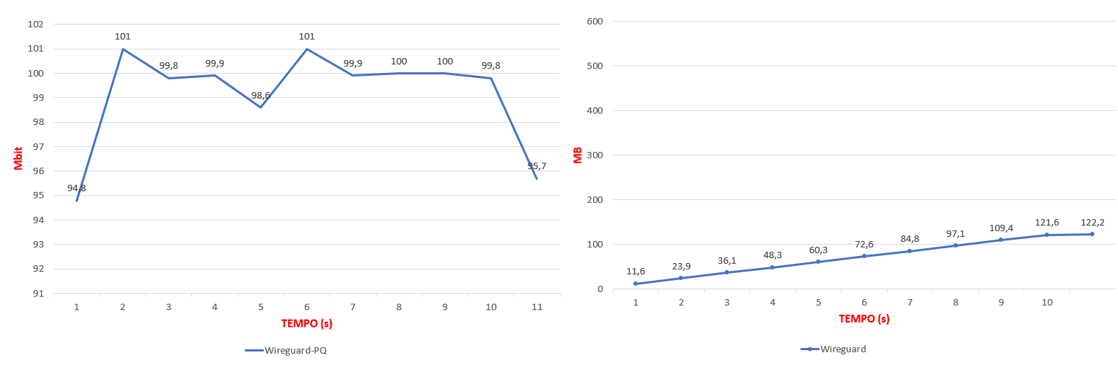
\includegraphics[width=0.9\textwidth] {Tesi magistrale/capitoli/images/33.png}
\centering
\caption{Grafici 1° esecuzione.}
\end{figure}

\begin{figure}[h] 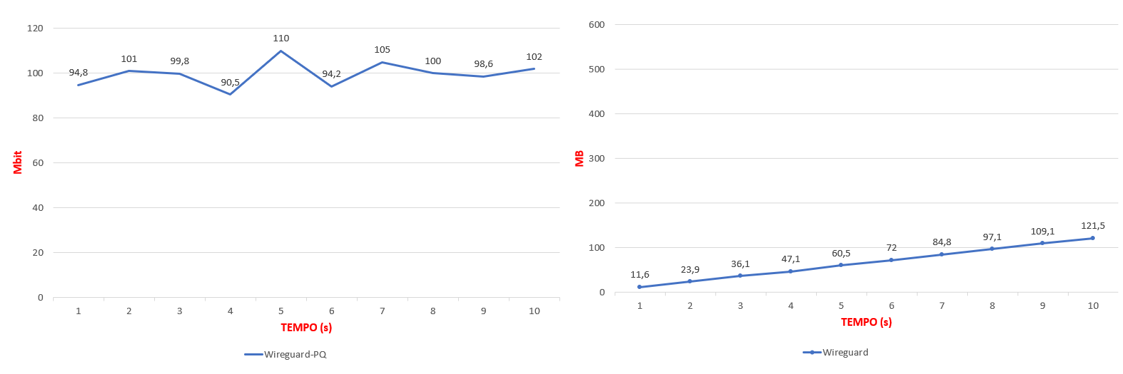
\includegraphics[width=0.9\textwidth] {Tesi magistrale/capitoli/images/34.png}
\centering
\caption{Grafici 5° esecuzione.}
\end{figure}

\begin{figure}[h] 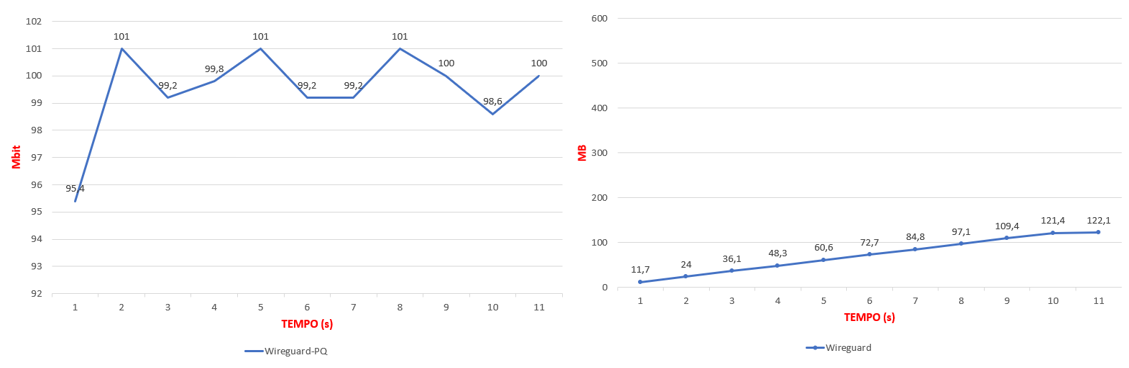
\includegraphics[width=0.9\textwidth] {Tesi magistrale/capitoli/images/35.png}
\centering
\caption{Grafici 10° esecuzione.}
\end{figure}

\newpage
\subsubsection{Grafici esperimento con OpenVPN}

\begin{figure}[h] 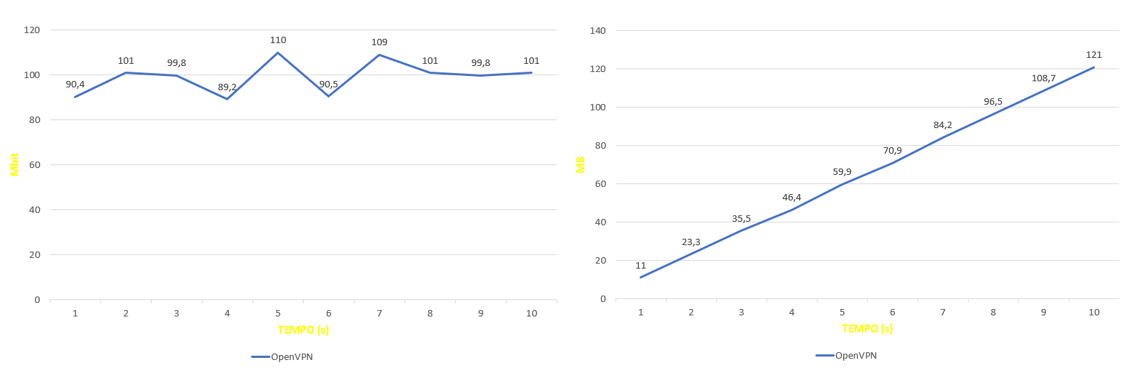
\includegraphics[width=0.9\textwidth] {Tesi magistrale/capitoli/images/42.png}
\centering
\caption{Grafici 1° esecuzione.}
\end{figure}

\begin{figure}[h] 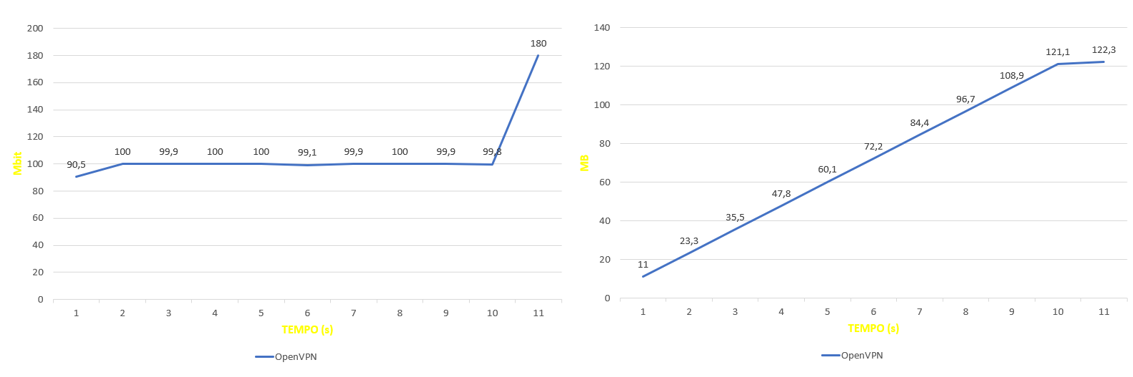
\includegraphics[width=0.9\textwidth] {Tesi magistrale/capitoli/images/43.png}
\centering
\caption{Grafici 5° esecuzione.}
\end{figure}

\begin{figure}[h] 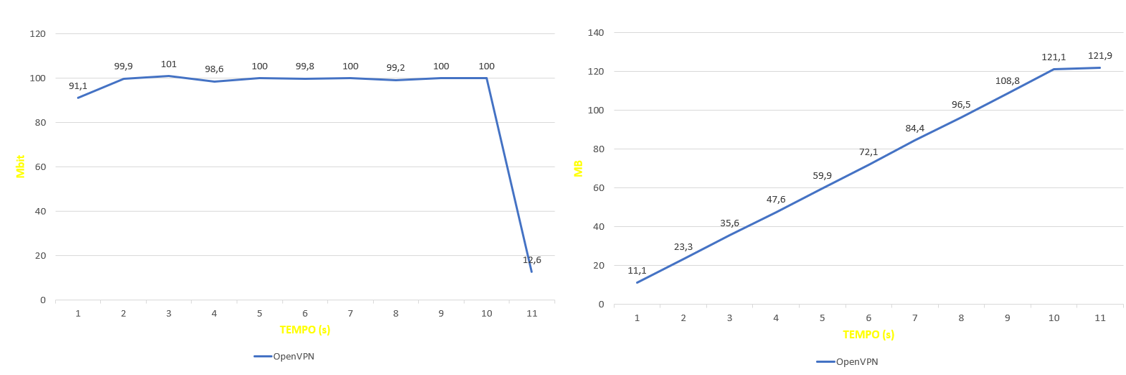
\includegraphics[width=0.9\textwidth] {Tesi magistrale/capitoli/images/44.png}
\centering
\caption{Grafici 10° esecuzione.}
\end{figure}

\newpage
\subsubsection{Grafici riassuntivi}

\begin{figure}[h] 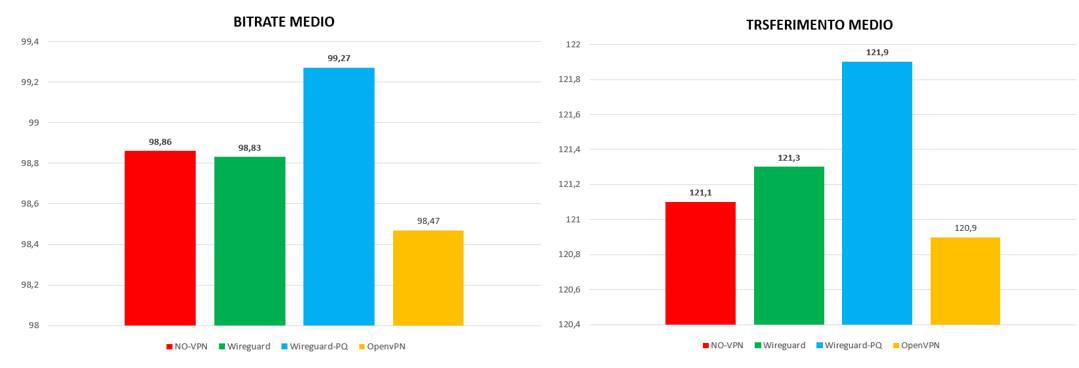
\includegraphics[width=1\textwidth] {Tesi magistrale/capitoli/images/36.png}
\centering
\caption{Grafici riassuntivi.}
\end{figure}

\subsubsection{Esito terzo esperimento}
Sorprendenmente nonostante il protocollo \emph{WireGuard PQ} sia oggettivamente più complesso data la sua natura, riesce, se pur leggermente, a sovrastare gli altri protocolli VPN testati e a superare addirittura l'esito del test senza l'utilizzo di VPN. 

\newpage
\subsection{Quarto esperimento}
Questo esperimento è stato ideato con l'obiettivo di simulare l'invio di pacchetti TCP appartenenti ad un flusso di dati adibito allo streaming video, come ad esempio \emph{Netflix}
\subsubsection{Grafici esperimento senza VPN}

\begin{figure}[h] 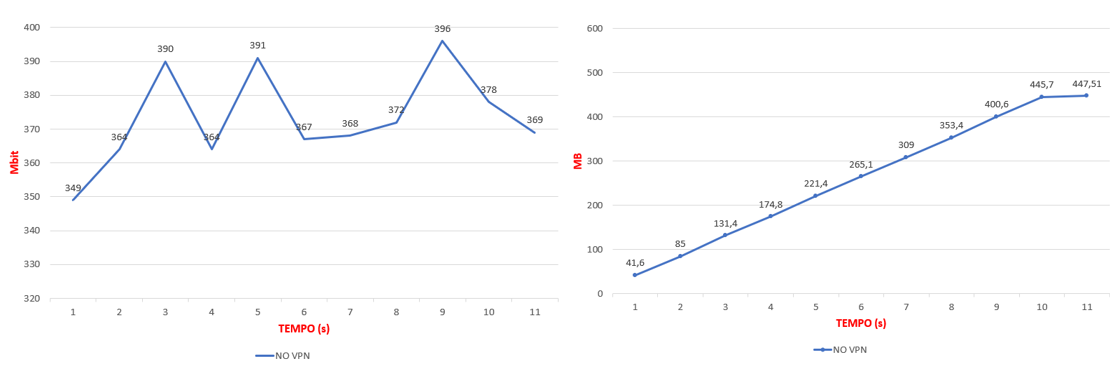
\includegraphics[width=0.9\textwidth] {Tesi magistrale/capitoli/images/37.png}
\centering
\caption{Grafici 1° esecuzione.}
\end{figure}

\begin{figure}[h] 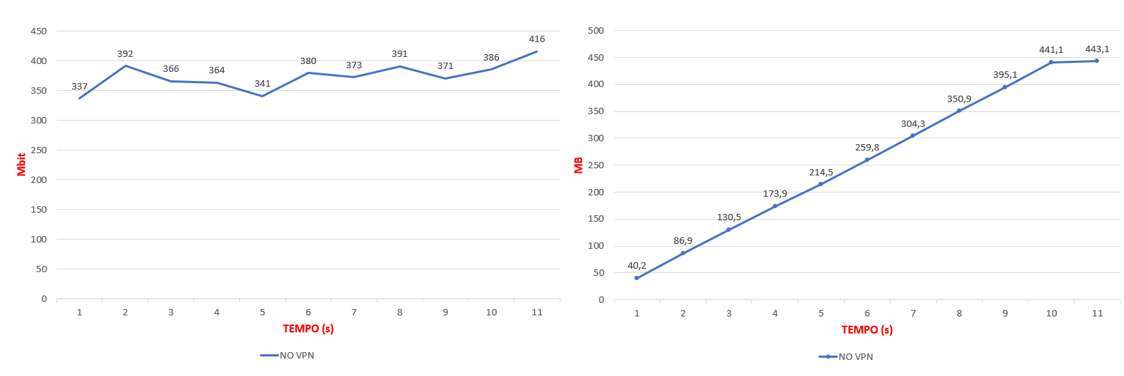
\includegraphics[width=0.9\textwidth] {Tesi magistrale/capitoli/images/38.png}
\centering
\caption{Grafici 5° esecuzione.}
\end{figure}

\begin{figure}[h] 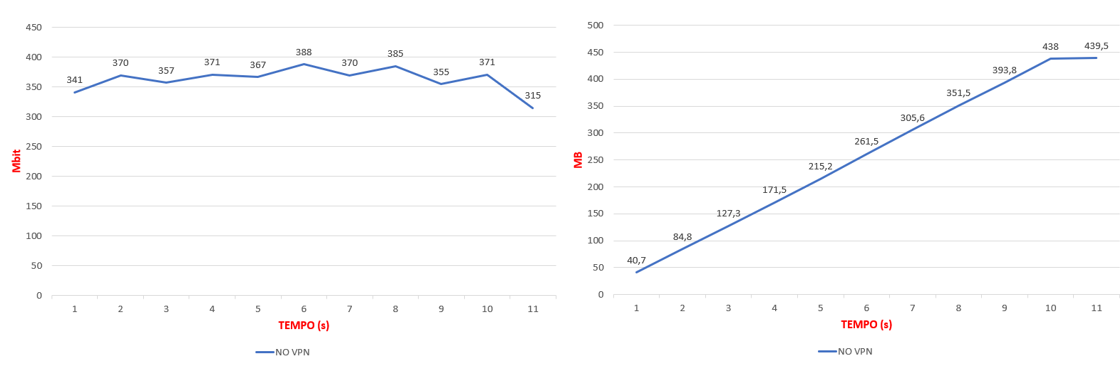
\includegraphics[width=0.9\textwidth] {Tesi magistrale/capitoli/images/39.png}
\centering
\caption{Grafici 10° esecuzione.}
\end{figure}

\newpage
\subsubsection{Grafici esperimento con WireGuard standard}

\begin{figure}[h] 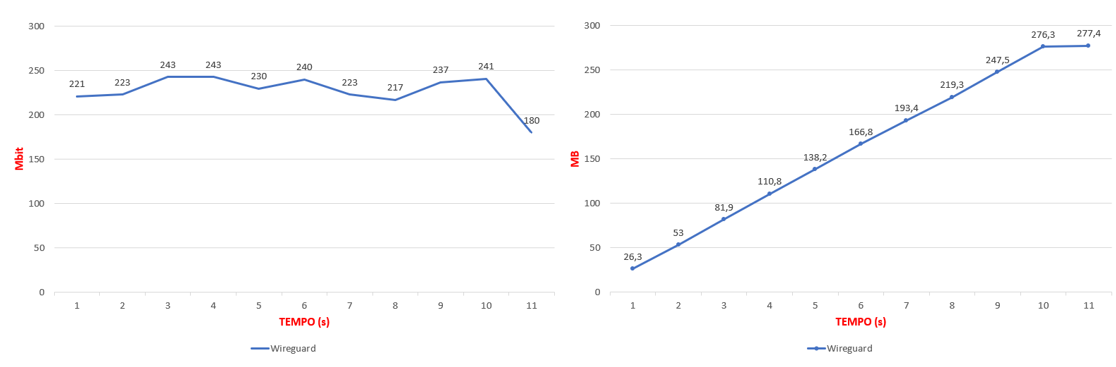
\includegraphics[width=0.9\textwidth] {Tesi magistrale/capitoli/images/40.png}
\centering
\caption{Grafici 1° esecuzione.}
\end{figure}

\begin{figure}[h] 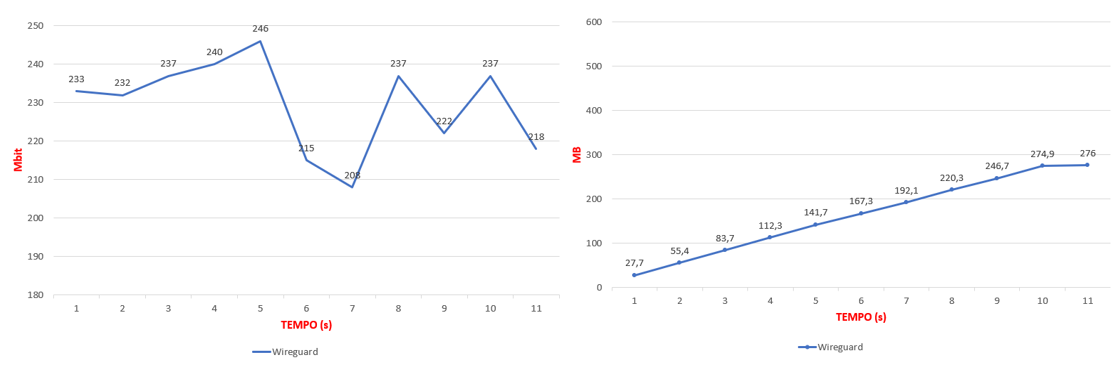
\includegraphics[width=0.9\textwidth] {Tesi magistrale/capitoli/images/41.png}
\centering
\caption{Grafici 5° esecuzione.}
\end{figure}

\begin{figure}[h] 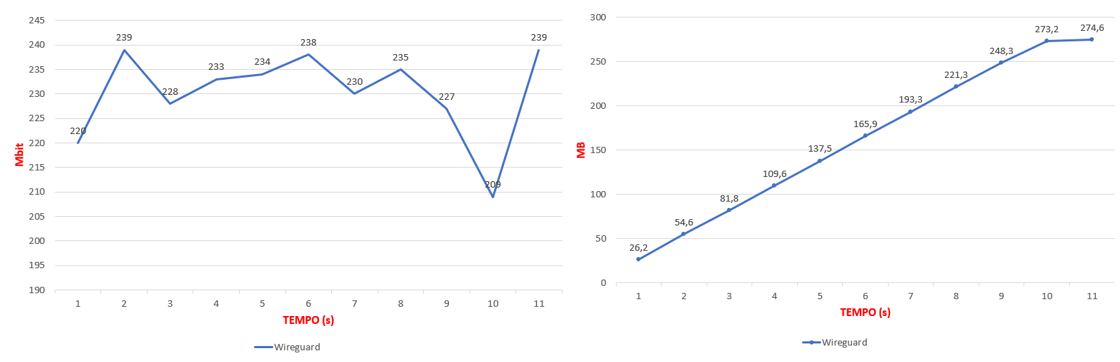
\includegraphics[width=0.9\textwidth] {Tesi magistrale/capitoli/images/45.png}
\centering
\caption{Grafici 10° esecuzione.}
\end{figure}

\newpage
\subsubsection{Grafici esperimento con WireGuard PQ}

\begin{figure}[h] 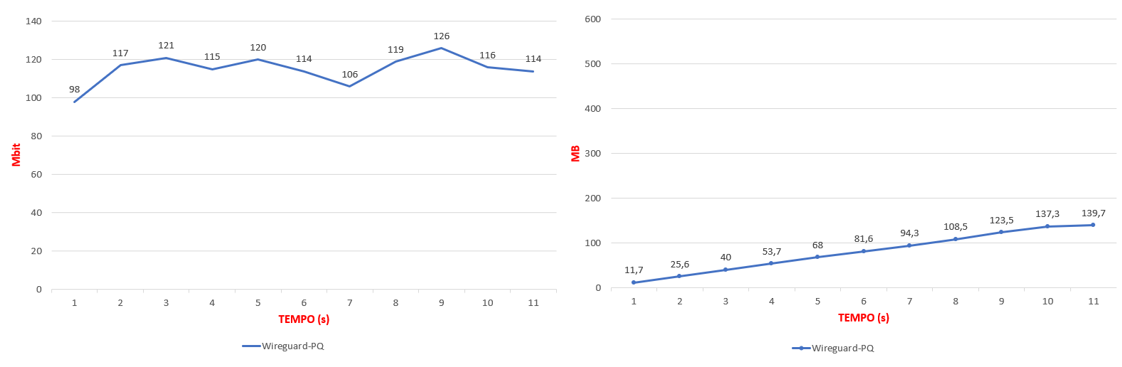
\includegraphics[width=0.9\textwidth] {Tesi magistrale/capitoli/images/46.png}
\centering
\caption{Grafici 1° esecuzione.}
\end{figure}

\begin{figure}[h] 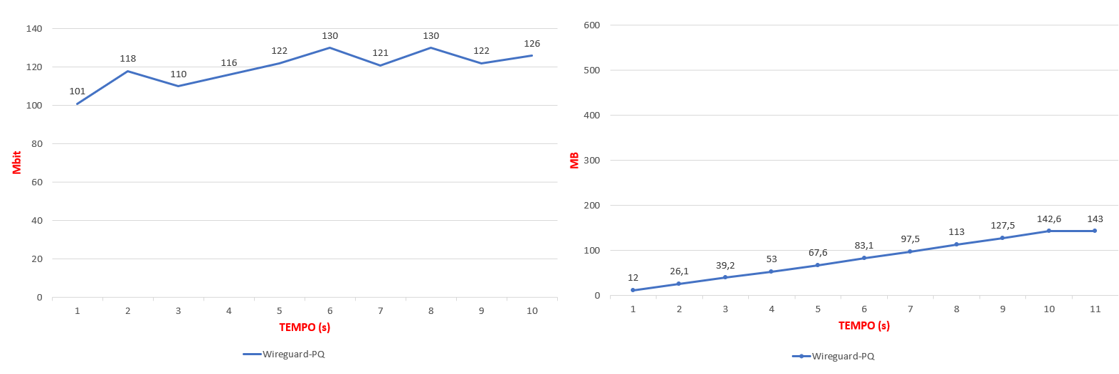
\includegraphics[width=0.9\textwidth] {Tesi magistrale/capitoli/images/47.png}
\centering
\caption{Grafici 5° esecuzione.}
\end{figure}

\begin{figure}[h] 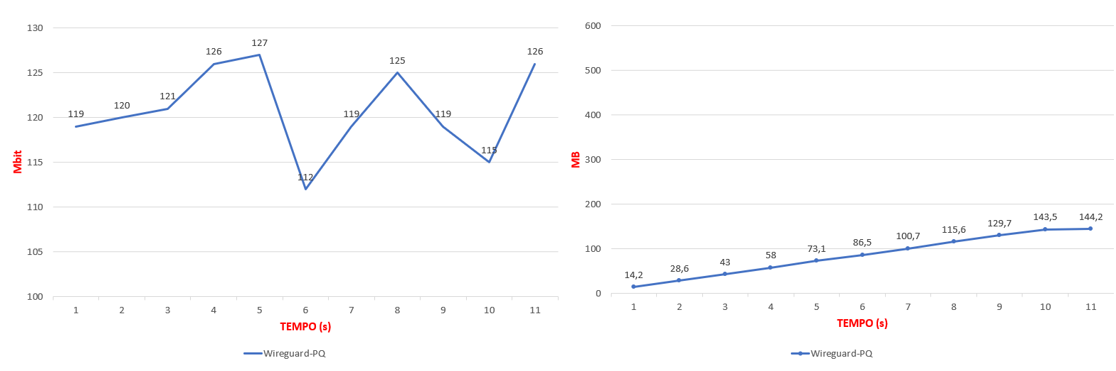
\includegraphics[width=0.9\textwidth] {Tesi magistrale/capitoli/images/48.png}
\centering
\caption{Grafici 10° esecuzione.}
\end{figure}

\newpage
\subsubsection{Grafici esperimento con OpenVPN}

\begin{figure}[h] \includegraphics[width=0.9\textwidth] {Tesi magistrale/capitoli/images/49.png}
\centering
\caption{Grafici 1° esecuzione.}
\end{figure}

\begin{figure}[h] \includegraphics[width=0.9\textwidth] {Tesi magistrale/capitoli/images/50.png}
\centering
\caption{Grafici 5° esecuzione.}
\end{figure}

\begin{figure}[h] \includegraphics[width=0.9\textwidth] {Tesi magistrale/capitoli/images/51.png}
\centering
\caption{Grafici 10° esecuzione.}
\end{figure}

\newpage
\subsubsection{Grafici riassuntivi}

\begin{figure}[h] \includegraphics[width=1\textwidth] {Tesi magistrale/capitoli/images/52.png}
\centering
\caption{Grafici riassuntivi.}
\end{figure}

\subsubsection{Esito quarto esperimento}
Per quanto riguarda questo esperimento, il comportamento migliore è stato ottenuto senza l'impiego di protocolli VPN mentre con essi sono stati ottenuti dei risultati che dimostrano chiaramente che la differenza prestazionale è abbastanza ampia, soprattutto se si considerano i protocolli \emph{WireGuard PQ} e \emph{OpenVPN}.

\newpage
\subsection{Quinto esperimento}
l'ultimo esperimento eseguito riguarda il trasferimento massivo di dati, in particolare i pacchetti appartengono ad un flusso di trasferimento massivo di tipo TCP.

\subsubsection{Grafici esperimento senza VPN}

\begin{figure}[h] \includegraphics[width=0.9\textwidth] {Tesi magistrale/capitoli/images/53.png}
\centering
\caption{Grafici 1° esecuzione.}
\end{figure}

\begin{figure}[h] \includegraphics[width=0.9\textwidth] {Tesi magistrale/capitoli/images/54.png}
\centering
\caption{Grafici 5° esecuzione.}
\end{figure}

\begin{figure}[h] \includegraphics[width=0.9\textwidth] {Tesi magistrale/capitoli/images/55.png}
\centering
\caption{Grafici 10° esecuzione.}
\end{figure}

\newpage
\subsubsection{Grafici esperimento con WireGuard standard}

\begin{figure}[h] \includegraphics[width=0.9\textwidth] {Tesi magistrale/capitoli/images/56.png}
\centering
\caption{Grafici 1° esecuzione.}
\end{figure}

\begin{figure}[h] \includegraphics[width=0.9\textwidth] {Tesi magistrale/capitoli/images/57.png}
\centering
\caption{Grafici 5° esecuzione.}
\end{figure}

\begin{figure}[h] \includegraphics[width=0.9\textwidth] {Tesi magistrale/capitoli/images/58.png}
\centering
\caption{Grafici 10° esecuzione.}
\end{figure}

\newpage
\subsubsection{Grafici esperimento con WireGuard PQ}

\begin{figure}[h] \includegraphics[width=0.9\textwidth] {Tesi magistrale/capitoli/images/59.png}
\centering
\caption{Grafici 1° esecuzione.}
\end{figure}

\begin{figure}[h] \includegraphics[width=0.9\textwidth] {Tesi magistrale/capitoli/images/60.png}
\centering
\caption{Grafici 5° esecuzione.}
\end{figure}

\begin{figure}[h] \includegraphics[width=0.9\textwidth] {Tesi magistrale/capitoli/images/61.png}
\centering
\caption{Grafici 10° esecuzione.}
\end{figure}

\newpage
\subsubsection{Grafici esperimento con OpenVPN}

\begin{figure}[h] \includegraphics[width=0.9\textwidth] {Tesi magistrale/capitoli/images/62.png}
\centering
\caption{Grafici 1° esecuzione.}
\end{figure}

\begin{figure}[h] \includegraphics[width=0.9\textwidth] {Tesi magistrale/capitoli/images/63.png}
\centering
\caption{Grafici 5° esecuzione.}
\end{figure}

\begin{figure}[h] \includegraphics[width=0.9\textwidth] {Tesi magistrale/capitoli/images/64.png}
\centering
\caption{Grafici 10° esecuzione.}
\end{figure}

\newpage
\subsubsection{Grafici riassuntivi}

\begin{figure}[h] \includegraphics[width=1\textwidth] {Tesi magistrale/capitoli/images/65.png}
\centering
\caption{Grafici riassuntivi.}
\end{figure}

\subsubsection{Esito quinto esperimento}
Anche in questo caso, come per diversi altri esperimenti, è evidente che l'utilizzo di protocolli VPN possa influenzare 
notevolmente le prestazioni di rete disponibili, spesso causando un decremento notevole come ad esempio nel caso del test eseguito con il protocollo \emph{OpenVPN}.